\vspace{-1.5cm}
\subsection{Visualising Process Model Forecasts}\label{sec:visualisation}

In~\Cref{sec:4.3:results}, we evaluated forecasting results, ensuring the conformance and interpretability of the predicted process models. To that end, gaining insights from such predicted data remains a difficult task for the analyst. 
This section sets off to present a novel visualisation system to aid analysts in exploring the event logs. The process of designing and implementing the system started by designing several prototypes that undergone rounds of discussions to mature into the implemented visualisation system. 

The design of the PCE system is shown in Figure~\ref{fig:vis-two-brushes}. It offers an interactive visualisation system with several connected views. The system is implemented using the D3.js JavaScript library and is available as an open-source project\footnote{See \url{https://github.com/yesanton/Process-Change-Exploration-Visualizations}}.

\begin{figure}
	\centering
	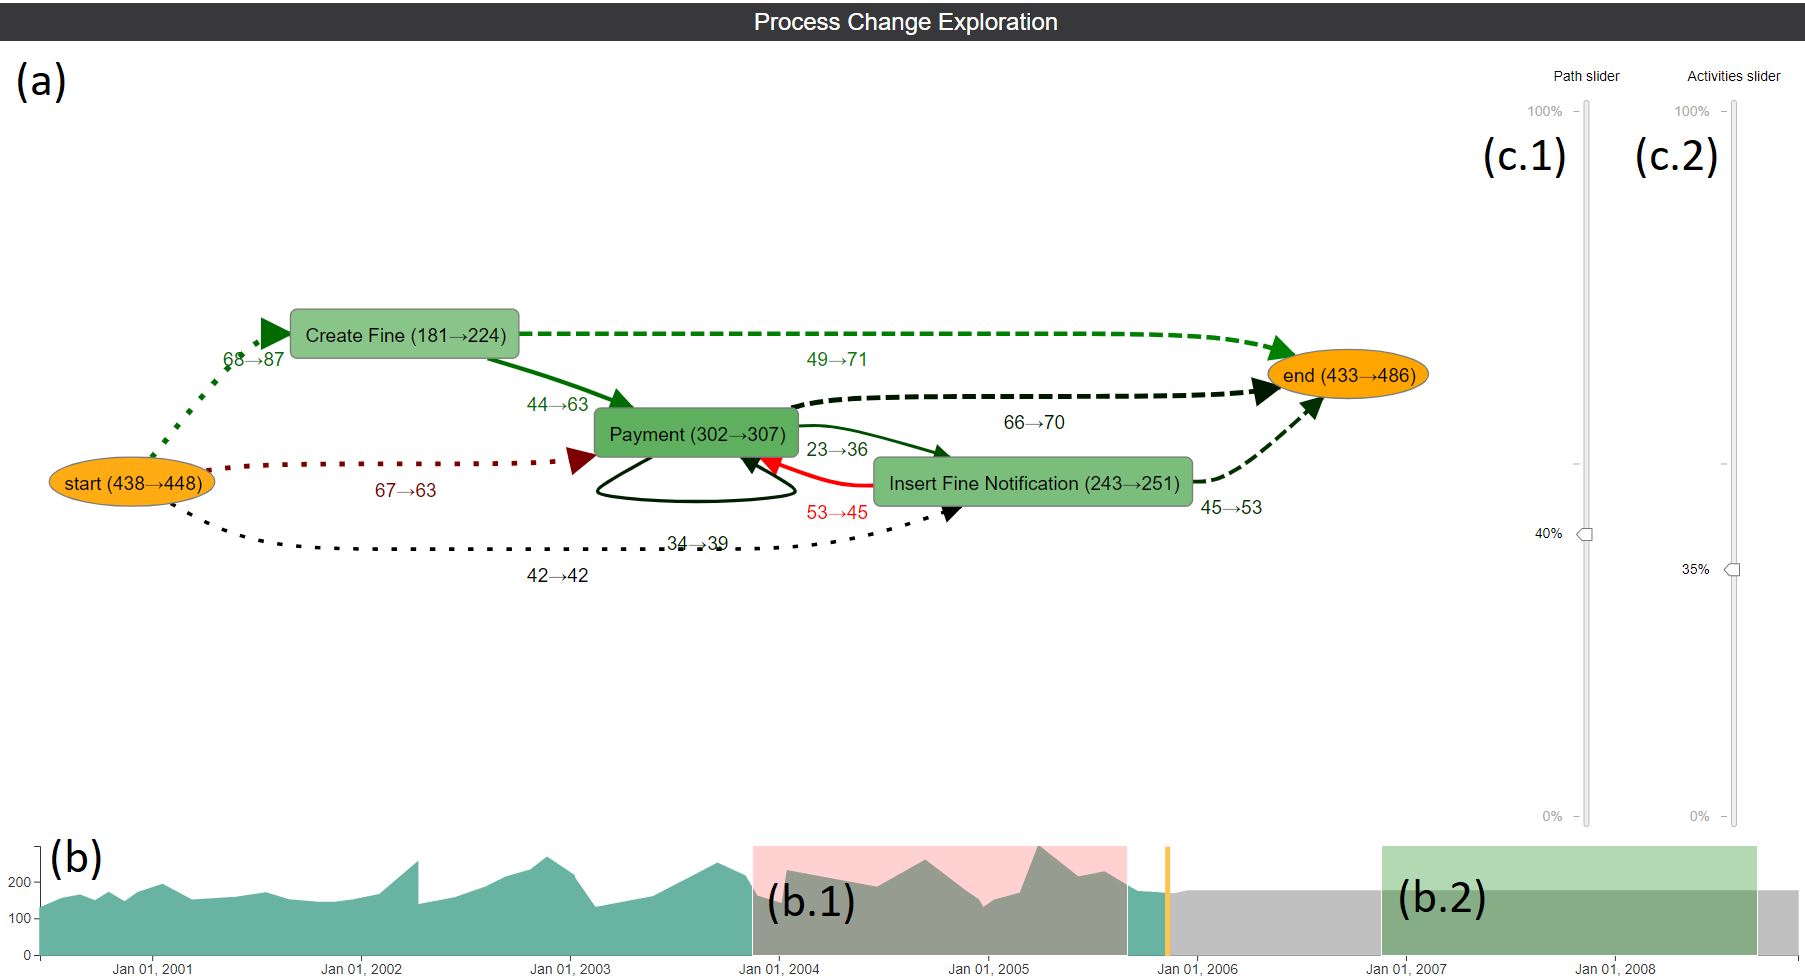
\includegraphics[width=\textwidth]{img/vis/actual-predicted-two-brushed-regions-system.PNG}
	\caption{Process Change Exploration (PCE) system.~\emph{(a)} shows~\emph{Adaptation Directly-Follows Graph (aDFG)} view.~\emph{(b)} shows the \emph{Timeline view with brushed regions} view. Users can brush one or more regions on this graph in order to filter the scope of the analysis~\emph{(b.1}, and~\emph{b.2)}. Two additional views on~\emph{(c)} show the \emph{activity and path sliders}.} 
	\label{fig:vis-two-brushes}
\end{figure}